%%
%% This is file `acmtog.tex',
%% generated with the docstrip utility.
%%
%% The original source files were:
%%
%% samples.dtx  (with options: `all,acmtog')
%% 
%% IMPORTANT NOTICE:
%% 
%% For the copyright see the source file.
%% 
%% Any modified versions of this file must be renamed
%% with new filenames distinct from acmtog.tex.
%% 
%% For distribution of the original source see the terms
%% for copying and modification in the file samples.dtx.
%% 
%% This generated file may be distributed as long as the
%% original source files, as listed above, are part of the
%% same distribution. (The sources need not necessarily be
%% in the same archive or directory.)
%%
%%
%% Commands for TeXCount
%TC:macro \cite [option:text,text]
%TC:macro \citep [option:text,text]
%TC:macro \citet [option:text,text]
%TC:envir table 0 1
%TC:envir table* 0 1
%TC:envir tabular [ignore] word
%TC:envir displaymath 0 word
%TC:envir math 0 word
%TC:envir comment 0 0
%%
%% The first command in your LaTeX source must be the \documentclass
%% command.
%%
%% For submission and review of your manuscript please change the
%% command to \documentclass[manuscript, screen, review]{acmart}.
%%
%% When submitting camera ready or to TAPS, please change the command
%% to \documentclass[sigconf]{acmart} or whichever template is required
%% for your publication.
%%
%%
\documentclass[acmtog,nonacm]{acmart}
%%
%% \BibTeX command to typeset BibTeX logo in the docs
\AtBeginDocument{%
  \providecommand\BibTeX{{%
    Bib\TeX}}}

%%
%% For managing citations, it is recommended to use bibliography
%% files in BibTeX format.
%%
%% You can then either use BibTeX with the ACM-Reference-Format style,
%% or BibLaTeX with the acmnumeric or acmauthoryear sytles, that include
%% support for advanced citation of software artefact from the
%% biblatex-software package, also separately available on CTAN.
%%
%% Look at the sample-*-biblatex.tex files for templates showcasing
%% the biblatex styles.



%%
%% end of the preamble, start of the body of the document source.
\begin{document}

%%
%% The "title" command has an optional parameter,
%% allowing the author to define a "short title" to be used in page headers.
\title{E-AI Data Gap Analysis: Understanding Data Barriers to ML-Driven Work in European Meteorological Services}

%%
%% The "author" command and its associated commands are used to define
%% the authors and their affiliations.
%% Of note is the shared affiliation of the first two authors, and the
%% "authornote" and "authornotemark" commands
%% used to denote shared contribution to the research.
\author{E-AI Working Group on Data Curation, https://github.com/eumetnet-e-ai/wg1_data_curation}

%%
%% The abstract is a short summary of the work to be presented in the
%% article.
\begin{abstract}
\end{abstract}

%%
%% This command processes the author and affiliation and title
%% information and builds the first part of the formatted document.
\maketitle
.\
\section{Introduction}
The E-AI Working Group on Data Curation conducted a Gap Analysis to better understand data-related obstacles preventing or slowing down ML-driven work across European National Meteorological and Hydrological Services, predominantly. This report summarises the key findings of the analysis and provides evidence-based recommendations to help accelerate and streamline future development efforts.

\section{Method}
The Gap Analysis included collection of data via GitHub, presentations and discussions in the working group, as well as a series of structured interviews between October to December 2025 with experts in the fields of weather and climate. A structured questionnaire was collaboratively designed to capture information on data challenges preventing or slowing domain experts' ML-driven workflows. A request was emailed to over 400 E-AI members for voluntary participation in a one-hour interview, in which the questionnaire was to be completed jointly between interviewer and interviewee. 

In each session, the interviewer and interviewee were shadowed by a third party taking notes wherever possible. Respondents rated data challenges by severity: minor for unavoidable inconveniences, significant for challenges solvable with time or resources, and blocker for challenges severe enough to prevent use of the data or to require a change in plan. Several questions were designed to be similar to one another to capture nuance. Respondents also rated preferred data formats and contributed to a ‘wish-list’. 

A live poll conducted at the E-AI Spring Meeting in Zagreb (n=42) independently replicated the core patterns from the interviews, providing confidence that the structured sample reflects a broader community experience. Results are included as supplementary.


\section{Results and Discussion}

\subsection{Respondent Profile}
\label{sec:subsection}
Eighteen domain experts participated, drawn from eleven EUMETNET member states (Belgium, Czechia, Denmark, Finland, France, Germany, Ireland, Portugal, Spain, Switzerland, and the UK) plus two private-sector organisations, IBM and Innoflair. Respondents' expertise spanned nowcasting and forecasting (n=10), climate (n=3), and operational products and services (n=5). Years of hands-on ML experience ranged from under two years to over ten. Fourteen participants used satellite data as a primary or co-primary source. Notably, most medium-term weather forecasting teams were not reached for interview and are hence not well-represented in these results.   
\label{sec:subsection}

\subsection{Data Challenges slowing ML-driven development}
\label{sec:subsection}

\begin{figure}[h]
  \centering
 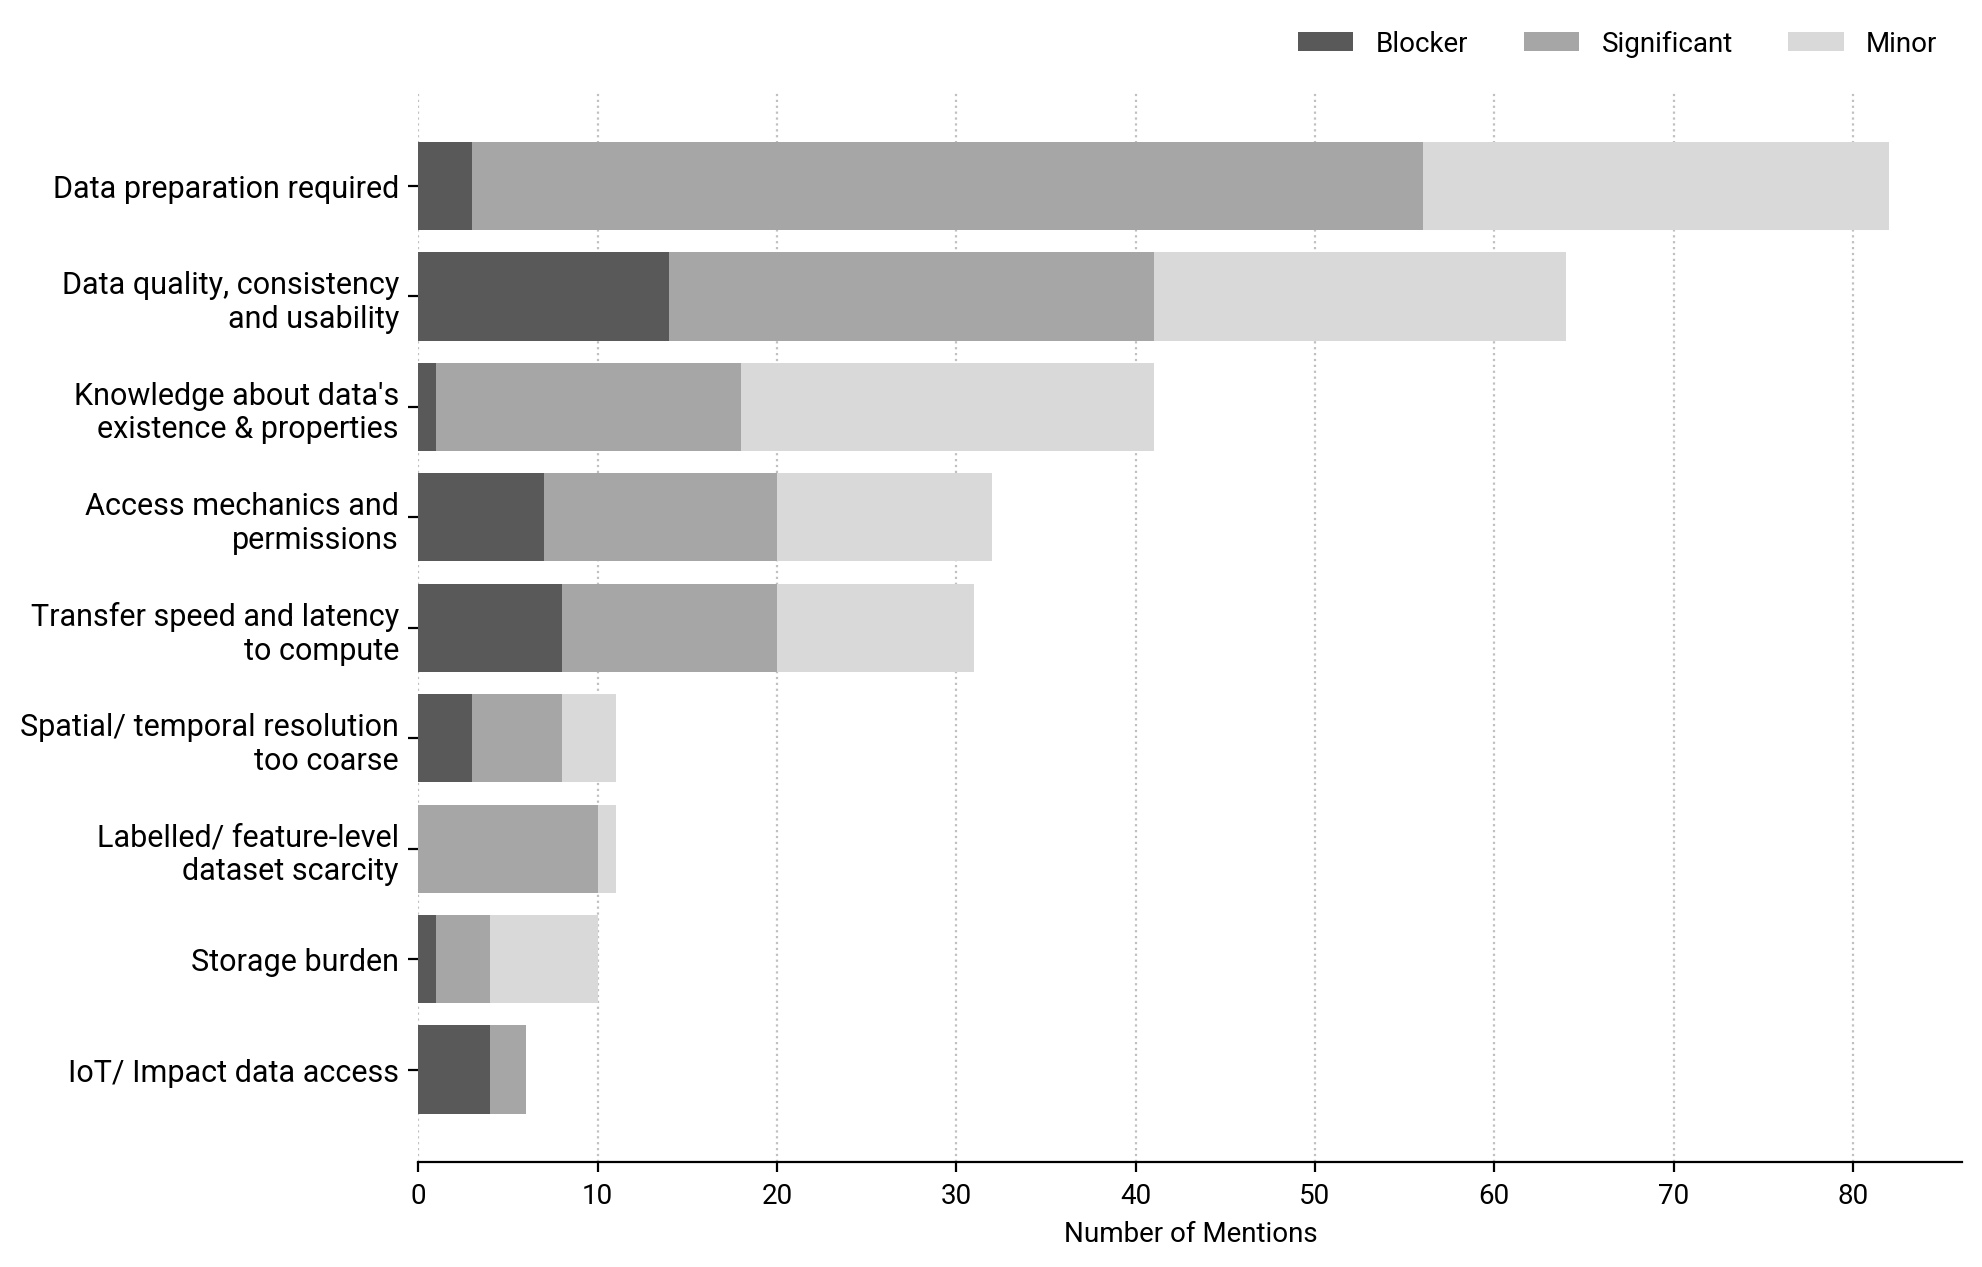
\includegraphics[width=\linewidth]{cluster_severity_chart}
  \caption{Heatmap of aggregated data-related challenges to ML-driven work across 18 interviews with respondent answers shaded by severity (blocker darkest to minor in lightest grey).}
  \Description{Histogram of clustered counts.}
\end{figure}

\subparagraph{\textbf{Data Challenges for EO vs non-EO data users:}}
\begin{itemize}
\item {\texttt{Users of EO satellite data (n=14)}}: slow download speeds and data format incompatibility were flagged as top challenges. Inconsistent formatting between organisations as well as complexity of geo-referencing and/or projections were also more problematic for this group.
\item{\texttt{Users of model output, ground observations, IoT (n=4)}}: storage burden was the dominant challenge for this cohort. Slow download speeds were flagged, however, uncertainty about what data products exist, unclear metadata, and data latency were raised as more prominent challenges.
\end{itemize}

\subparagraph{\textbf{Data Challenges by Application Areas:}}
\begin{itemize}
\item {\texttt{Nowcasting and forecasting (n=10)}}: defining concerns were data continuity (time-series gaps and missing data content) and speed (slow download speeds and moving data close to compute). Lack of expert-labelled datasets was flagged by 7/10 respondents.
\item {\texttt{Climate (n=3)}}: All respondents flagged slow download speeds (blocking for 2/3), data formats, pre-processing, limited labelled datasets, complex /missing geo-referencing as challenges. Large differences between training and inference data were also blocking for two respondents.
\item{\texttt{Products and services (n=5)}}: uncertainty about what data products exist was flagged by all five respondents. Data structured unsuitably for the use case and large training/ inference discrepancies were blocking for 2/5. 
\end{itemize}
.\\
\subparagraph{{\textbf{A Note on Frequent vs Severe Data Challenges:}}}
Results from this Gap Analysis also highlight two meaningful categories of data challenges for ML-driven work – frequency and severity.
\begin{itemize}
\item {\texttt{Frequency }} e.g. data preparation steps required before data are suitable for ML was flagged by all respondents, regardless of application area, experience level, or data source. While this challenge is rarely a block, it is slowing down development for users across the board.
\item {\texttt{Severity }}e.g. data quality and consistency challenges (including large differences between training and inference data), speed and data latency (including slow data download speeds), and access friction forced around 25\% of respondents to abandon or change their planned workflow. Both categories must be addressed to speed up development.
\end{itemize}

\subsection{Specific Data Challenges}
\label{sec:subsection}

\subparagraph{\texttt{Data preparation requirements}}
:\newline
The requirement for data to be reprocessed, reformatted, and/or reprojected before being ready for ML is a frequent bottleneck for development teams, and ~65\% of respondents rated data preparation as a significant challenge. The problem is frequent but may not be entirely unavoidable as most applications are different. 

Ratings here, as well as with overcoming access-challenges, reflect what has impacted the person answering the questionnaire, not necessarily what is experienced at an organisational level. Some respondents rated a data access challenge as minor or absent because a dedicated team absorbs it. Interviewees from data management in the same organisation described access friction as “part of our job” — mitigating what would otherwise be severe access challenges. A counter-example is a smaller, newer team building nowcasting models from scratch. In this case, substantial friction was reported for the same categories, likely because there is team in place yet to absorb it. Thus, it may be that bigger/ better-resourced organisations do not have smaller problems, rather that they have more resources between them and data access challenges.

Although data preparation/ reformatting is a persistent, significant friction for every development team, this challenge is unlikely to be entirely avoidable as most applications are different. Nevertheless, if undifferentiated parts of the preparation – e.g. reprojecting, reformatting, and quality control – can be centralised, the community can empower developers from smaller organisations and save significantly especially in terms of expert time also in bigger organisation.

\subparagraph{\texttt{Accessing storing data}}
:\newline
Biggest source of blockers, causing teams to change their plans or preventing them to do the research they wanted, was related to transferring and storing large amount of data. Large data volumes often became a practical barrier before model development can even begin. Slow downloads made some data acquisitions impractical, and in one example, the estimated download time for the required IFS dataset was longer than the duration of the project. Moving data between local computers, institutional storage, HPC and GPU environments was likewise described as slow. Storage added a further constraint: limited capacity forced teams to retain only samples, while also large numbers of Zarr objects caused challenges. Together, these findings indicate a need for reliable high-volume online storage architectures suited to ML data structures, and analysis-ready datasets hosted close to the computing resources on which they will be used.

Data-policy issues were reported primarily as licensing and sharing barriers. Some teams could use data internally but could not openly redistribute training data with their project partners, limiting reproducibility, publication, and community reuse. Commercial licences prevented use of some satellite and impact datasets, while differing or non-standard licences complicated the creation of combined multi-source datasets. Interviewees also identified bureaucracy and permission processes as access barriers. Future shared data cubes and labelled datasets therefore require clear, preferably standardised terms covering source-data processing, derived products, annotations, model training and redistribution within the community.

\subparagraph{\texttt{Data quality, consistency, usability}} 
:\newline
Data quality issues were mentioned as a major challenge, especially for station and ground sensor observations, but this was not a frequent challenge. Instead, lack of homogenous, and gap-free high-quality long time-series as well as drift and inconsistencies within time-series were often mentioned as severe (a blocker). Other challenges, such as data latency and differences between training and inference material, were marked sometimes as a block, and sometimes as a minor challenge with an explicit qualifier: “not [problematic] at the moment”. One respondent noted that data latency was not an issue for the climate version of a project, but “will be an issue” once it shifts to nowcasting. Another team described current comfort as conditional: latency “will be vital, once we move to operation - that will be the most critical thing”. 

This underlines two key considerations: development teams need to design the operational setup from the beginning of the project, but also data providers should prioritise long-term continuation of the data including similar-enough archive and real-time data access, especially as many meteorological applications have been proven to benefit from decades of training data.

\subparagraph{\texttt{•	Knowledge about data’s existence and properties}} 
:\newline
Users often struggle to determine which datasets exist, where they are located, and whether their properties make them suitable for a particular application. Discoverability was hindered by fragmented catalogues and access points, inconsistent terminology, and limited awareness even among experienced users. These findings point to the need for application-aware data curation for both human and agents that describe not only the existence and location of data but also help choosing the correct content and support in its preparation.  


\subsection{Data Format Preferences}
\label{sec:subsubsection}
The interview respondents rated preferred data formats on a scale of 1 (least preferred) to 5 (preferred); several used negative scores to express strong rejection. The table below reflects directional sentiment rather than precise averages.

\begin{figure}[h]
  \centering
 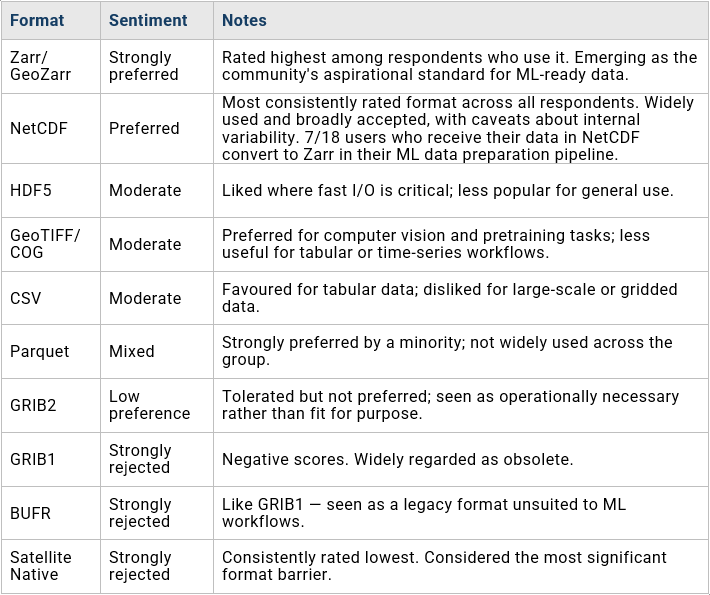
\includegraphics[width=\linewidth]{GA_dataformat_preff.png}
  \caption{ Table showing the most preferred and least preferred data format options with notes for insights into what is driving user sentiments.}
  \Description{Table of data format preferences.}
\end{figure}
From the responses, direction of travel appears to show a ML community moving to cloud-native, chunked, analysis-ready formats that suit ML pipelines directly without additional reformatting. The gap between what is currently disseminated and what ML users prefer (Zarr, NetCDF, cloud-optimised) is a concrete area where data providers can reduce access friction and downstream reformatting / processing load.

\subsection{Data Wish List}
\label{sec:subsubsection}
Interview respondents were asked to identify data/sets and products that would most enhance their ML work. Across 18 respondents, over 50 specific items were submitted, clustering into five principal themes:

\begin{itemize}
\item {\texttt{Expert-labelled feature datasets}}: most frequently cited, especially in nowcasting and forecasting group. Desired features included overshooting tops, mesoscale convective systems, fire features, seaweed and harmful algal blooms, clear air turbulence, icebergs, and radar weather features. Respondents wished for curated, open datasets with consistent labelling standards. 
\item{\texttt{Analysis-ready cloud-optimised}}: Respondents wished that current EUMETSAT data and products were reprojected onto consistent grids, chunked in space and time, with consistently named variables, i.e.: data that can be consumed directly by ML pipelines without reformatting.
\item {\texttt{Gap-free high quality long time series}}: Respondents using ground-based radar and other station data wished for longer more consistent records (pre-2010), standardised meteorological data with complete metadata, consistent aggregation, and documented fill values.
\item {\texttt{Impact and IoT data}}: Respondents wished for open, event-based impact data collated with weather observations (fires, floods, storms, power outages). Those who need Impact and IoT data were a minority, but lack of access here significantly limits their ML work (very high blocker rate).
\end{itemize}


\section{Recommendations}

\subparagraph{\texttt{Provide commonly used datasets as analysis-ready Zarr data cubes with high-performance community access of undifferentiated parts of the pipeline to remove the data preparation burden from development teams }} 
:\newline
While virtual Zarrs, supporting libraries, and on-demand services may be sufficient where users still need to perform application-specific preparation, the gap analysis also identified cases where multiple teams and applications can use the same prepared data directly. For these cases, as well as when data are exceptionally distributed or complicated, centrally maintained data cubes are justified, even at the cost of some data duplication.

The amount of variety in solutions need to be balanced, carefully listening to the development teams. Multiple relevant initiatives already exist within the community. ANEMOI has gained significant interest in the weather forecasting domain and provides a strong example of collaborative data preparation, data cataloguing, and efficient distribution of data across different environments. However, it is highly application-specific and should not be regarded as a universal solution. Activities such as DEFAIR and Firecube demonstrate the transition towards Zarr while continuing to serve user communities with wide range of applications, that may rely also on NetCDF- or TIFF-based workflows. MLCast is a great example of bottom-up community effort to collect and prepare distributed radar data and complicated satellite data to a centrally usable form.  

Across all such initiatives, data sovereignty and clear attribution remain essential. This is particularly important for data providers, whose ability to continue sharing data with the wider community depends on appropriate recognition, governance, and control over their contributions.

\subparagraph{\texttt{Raise long history of data from deep archives to commonly usable appropriate online access}} 
:\newline
To realise the benefits of prepared data cubes, data must be directly usable from the training environments via one or few copies of the dataset. This requires large-enough fast storage systems and appropriate access mechanisms (e.g. S3 interface) to enable synchronous data access. This need is one of the large changes in computing ecosystem requirements caused by machine-learning which is also evident in large number of blockages in the interviews. To address this, investments in storage are needed. In addition, it is important to move from asynchronous individual data exchange to community-driven collaboration around data.

\subparagraph{\texttt{Enforce community with active collaboration and circle of trust to ensure frictionless access to the data}} 
:\newline
To empower the community spanning across institutes and countries to jointly work on the data (including read and write), frictionless access to the data must be ensured. Beyond data preparation and infrastructure, “circle of trust” needs to be enforced, making sure that the community developers can freely and easily access all relevant data and they can share the prepared datasets within their (often international) projects. This requires careful governance to distinguish collaboration happening in the inner circle while keeping wider community open to fluent but managed interaction with e.g. private sector. Both EUMETNET E-AI and raising EMI Data Space for Weather and Climate are good vehicles to achieve these goals.

Active data curation is also needed to mitigate issues with knowledge about existing data and its properties. This includes a creation of application- and domain-aware data menu as well as activities such as Earth System Feature detection, supporting both labelled datasets and data discovery. Curation should also ensure that users know and manage to use the best available datasets for their task and that users can confidently combine, share and reuse them across applications. Notably, these efforts must be directed as much for agents as for humans.


\clearpage

\section{Supplementary Materials}

Eighteen domain experts from eleven EUMETNET member states participated in the Gap Analysis interviews. Notably, most medium-term weather forecasting teams were not reached for the interview and are hence not well-represented in these results. Anonymised individual responses to each question in the Data Challenges section are shown in Figure~\ref{fig:GapAnalysis_all}:

\begin{figure}[h!]
  \centering
 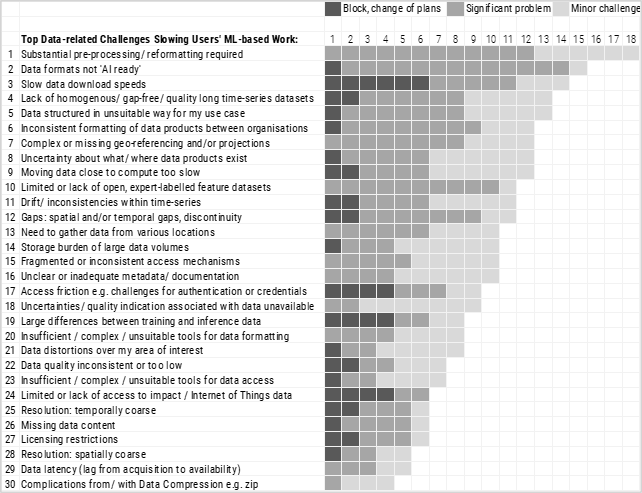
\includegraphics[width=\linewidth]{GA_individual_counts.png}
  \caption{Heatmap of granular data-related challenges to ML-driven work across 18 interviews with respondents’ answers shaded by severity (blocker darkest to minor in lightest grey).}
  \Description{Table of responses.}
  \label{fig:GapAnalysis_all}
\end{figure}

\begin{figure}[h]
  \centering
 
\includegraphics[width=\linewidth]{GA_aggregate_counts.png}
  \caption{Table of aggregated counts of data challenges grouped by theme (e.g. data preparation, quality, access, speed)}
  \Description{Table of responses.}
\end{figure}

\subsection{E-AI Spring Meeting Live Poll, Zagreb}
\label{sec:subsection}

At the E-AI Spring Meeting in Zagreb, a live Slido poll was conducted with approximately 70 attendees, covering primary data sources used, data challenges experienced, and preferred data formats. 57 participants responded; 42 provided complete answers to both the data sources and challenges questions and are included in Figure~\ref{fig:slido_heatmap}. The poll used binary flagging (flagged or not flagged) rather than the three-level severity coding used in the interviews, so frequency of mention is the primary metric.

Most respondents here did not use EO as their primary data source, however, the domain-level patterns from the interviews are broadly replicated in the live poll. Slow download speeds dominate for the climate group (71\%). Uncertainty about what data products exist is most prominent for products and services (50\%). Labelled dataset concerns remain concentrated in nowcasting/forecasting (33\%). Storage burden is the top challenge for the non-satellite group (68\%) and for products and services (67\%).

\begin{figure}[H]
  \centering
 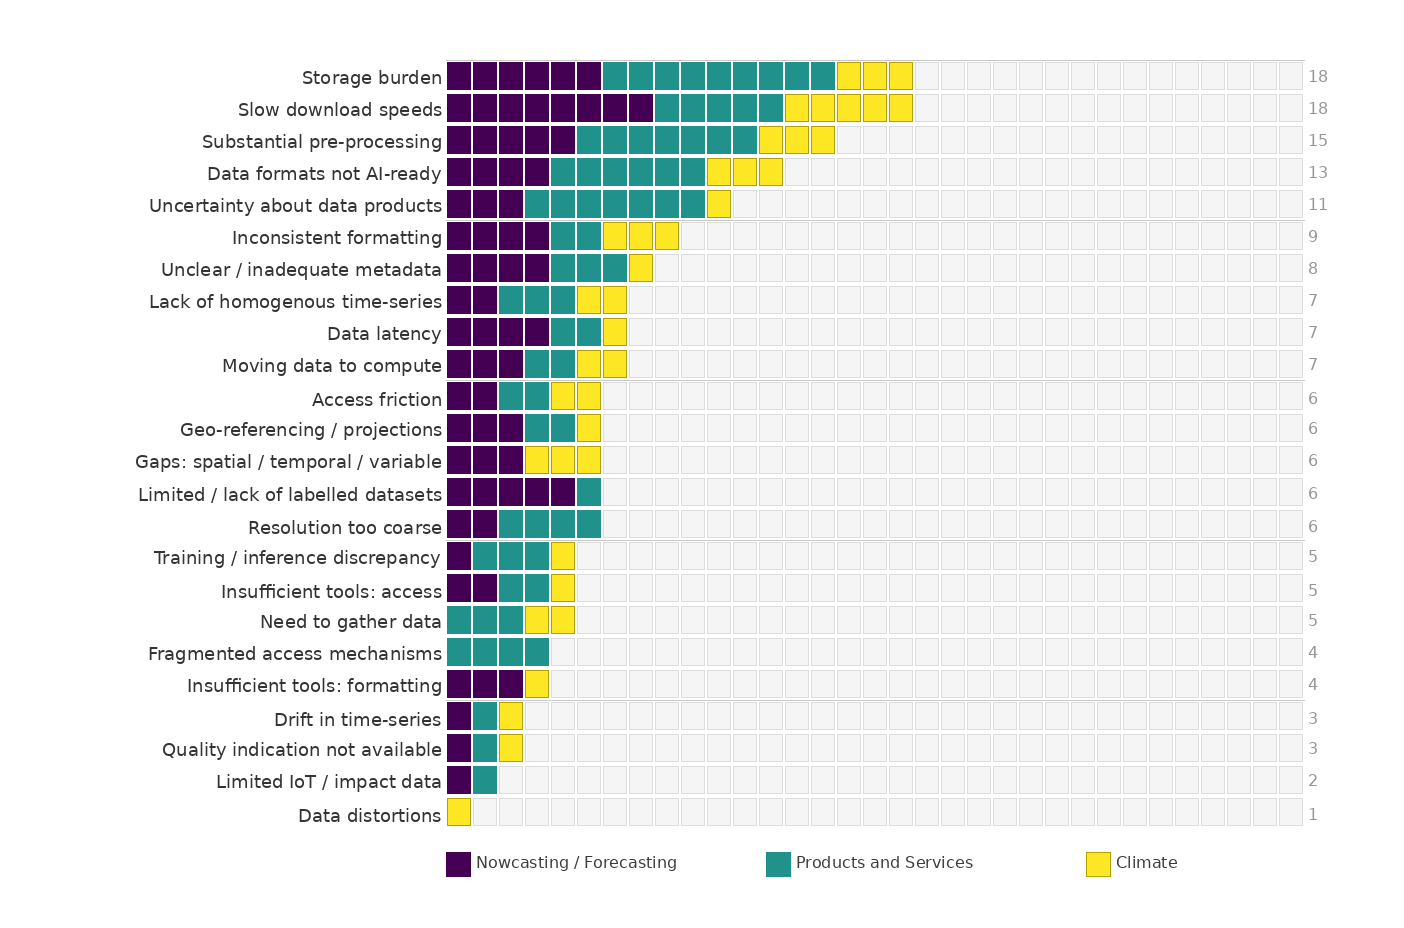
\includegraphics[width=\linewidth]{Zagreb_slido_counts.png}
  \caption{Live poll respondents (n=42 with complete domain and challenge data), grouped by primary application area.}
  \Description{Live poll heatmap}
  \label{fig:slido_heatmap}
\end{figure}

Zarr/GeoZarr and NetCDF were the most preferred formats among these respondents, consistent with the interview findings. GRIB1, BUFR, and satellite-native formats were the least preferred; CSV was preferred for tabular workflows. 

\end{document}
\endinput
%%
%% End of file `acmtog.tex'.
